\subsection{Enriched Semantic Event Chains}
\label{ssec:action_methods_enrichedsemanticeventchains}

As seen in the last chapter, for robot execution of Semantic Event Chains, some additional pose information must be included.
Therefore, \glspl{ac:sec} are enriched by higher level structural information.
Each entry of one keyframe matrix now may not only hold ``T'', ``N'', or ``A'', but also an additional vector containing the relative pose between the two objects.
An example can be seen in \figref{fig:sec_examplescenario_pushing_firstkeyframe}, which is similar to the first keyframe in the example \figref{fig:sec_examplescenario_pushing}, but introduces an additional coordinate system.
Following this approach, the Semantic Event Chain turns into an \gls{ac:esec} as

\begin{figure}
  \centering
  % Define block styles
\tikzstyle{block} = [rectangle, fill=white, text centered, minimum height=0.5em, rounded corners=true]
\tikzstyle{blockBox} = [draw, rectangle, fill=white, minimum height=2.8cm, minimum width=6.0cm, text width=1em, text centered, rounded corners=true]

\tikzstyle{blockSupP} = [draw, rectangle, fill=red1!20,   minimum height=0.52cm, minimum width=1.3cm, text width=1em, text centered, rounded corners=true]
\tikzstyle{blockSupM} = [draw, rectangle, fill=green1!20, minimum height=0.52cm, minimum width=3.1cm, text width=3.1cm, text centered, rounded corners=true]
\tikzstyle{blockSupS} = [draw, rectangle, fill=blue1!20,  minimum height=0.52cm, minimum width=1.3cm, text width=1em, text centered, rounded corners=true]
\tikzstyle{blockSup}  = [draw, rectangle, fill=red1!20,   minimum height=0.52cm, minimum width=3.1cm, text width=3.1cm, text centered, rounded corners=true]

\tikzstyle{blockCon} = [draw, rectangle, fill=white, minimum height=0.5cm, minimum width=1cm, text width=0.6cm, text centered, rounded corners=true]
\tikzstyle{blockP} = [draw, rectangle, fill=red1!40, minimum height=0.52cm, minimum width=0.6cm, text width=1em, text centered, rounded corners=true]
\tikzstyle{blockM} = [draw, rectangle, fill=green1!40, minimum height=0.52cm, minimum width=0.6cm, text width=1em, text centered, rounded corners=true]
\tikzstyle{blockS} = [draw, rectangle, fill=blue1!40, minimum height=0.52cm, minimum width=0.6cm, text width=1em, text centered, rounded corners=true]
\tikzstyle{blockL} = [draw, rectangle, fill=black!20, minimum height=0.52cm, minimum width=0.6cm, text width=1em, text centered, rounded corners=true]
\tikzstyle{arrow} = [draw, -latex]
\tikzstyle{line} = [draw]

\definecolor{red1}{RGB}{160,0,0}
\definecolor{green1}{RGB}{0,160,0}
\definecolor{blue1}{RGB}{0,0,160}

\pgfdeclareimage[width=0.6cm]{hand}{./figures/sec/robothand.jpg}

	      
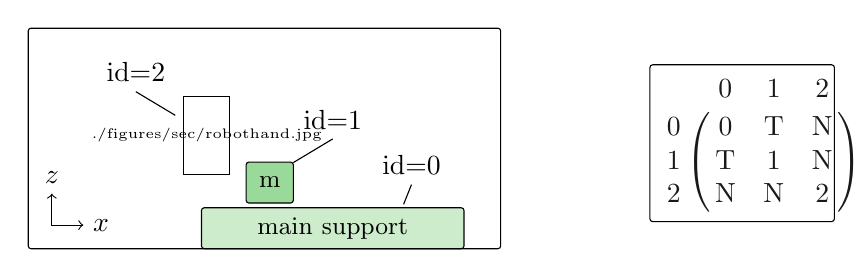
\begin{tikzpicture}[node distance=6em, auto]
	%%%%%%%%%%%%%%%%%%%%%%%%%%%%%%%%%%%%%%%%%%%%%%%%%%%%%%%%%%%%%%%%%%%%%%%%%%%%%%%%%%%%%%%%%%%%%%%%%%%%%%
	% Panel
	\node [blockBox] (p11) {};

	\node[above right, xshift=2.2cm, blockSupM, minimum width=3cm] at (p11.south west) (p11_Sup) {\small{main support}};
	\node[above of=p11_Sup, blockM, node distance=0.58cm, xshift=-0.8cm] (p11_m) {\small{m}};
	\node[left of=p11_m, node distance=0.8cm, yshift=0.6cm] (p11_h) {\pgfuseimage{hand}};

    % Text
    \node[right of=p11_Sup, node distance=0.8cm, xshift=0.2cm, yshift=0.8cm] (p11_Sup_t) {id=0};
    \node[right of=p11_m,   node distance=0.8cm, xshift=0.0cm, yshift=0.8cm] (p11_m_t) {id=1};
    \node[left of=p11_h,    node distance=0.8cm, xshift=-0.1cm, yshift=0.8cm] (p11_h_t) {id=2};

    % Lines
    \draw[line] (p11_Sup_t.south) to ++(-0.1cm,-0.25cm);
    \draw[line] (p11_m_t.south) to ++(-0.5cm,-0.3cm);
    \draw[line] (p11_h_t.south) to ++( 0.5cm,-0.3cm);

    \draw [<->] (-2.7cm,-0.7cm) node (yaxis) [above] {$z$}
                |- (-2.3cm,-1.1cm) node (xaxis) [right] {$x$};


	%%%%%%%%%%%%%%%%%%%%%%%%%%%%%%%%%%%%%%%%%%%%%%%%%%%%%%%%%%%%%%%%%%%%%%%%%%%%%%%%%%%%%%%%%%%%%%%%%%%%%%
	% Matrix

    \node[block, right of=p11_m, yshift=0.5cm, node distance=6.0cm] (p31) {
      $\bordermatrix{
          & 0 & 1 & 2\cr
        0 & 0           & \textup{T}    & \textup{N}\cr
        1 & \textup{T}  & 1             & \textup{N}\cr
        2 & \textup{N}  & \textup{N}    & 2\cr        
      }$
    };
\end{tikzpicture}

  \caption{This is the same scene as shown in \figref{fig:sec_examplescenario_pushing} --- a robot pushing the \emph{main} object along its support. Please note the coordinate system, which is used when the keyframe matrix on the right is enriched by relative pose information, see \eqnref{eqn:sec_enriched_2d}. For clarity only two dimensions are used here (where $y=0$).}
  \label{fig:sec_examplescenario_pushing_firstkeyframe}
\end{figure}

\begin{align}
  \bordermatrix{
    & 0 & 1 & 2\cr
    0 & \colorbox{green120}{0}    & (\textup{T},~(0,~0,~1))         & (\textup{N},~(0,~0,~1))\cr
    1 & (\textup{T},~(0,~0,~-1))  & \colorbox{green120}{1}          & (\textup{N},~(-0.71,~0,~0.71))\cr
    2 & (\textup{N},~(0,~0,~-1))  & (\textup{N},~(0.71,~0,~-0.71))  & \colorbox{green120}{2}\cr
    },
  \label{eqn:sec_enriched_2d}
\end{align}

where the ID is marked in green.
A more general form for the keyframe matrix $\underline{K}$ is

\begin{align}
  \underline{K} := \begin{pmatrix}
    a_{0,0}         & \vec{a}_{1,0} & \cdots & \vec{a}_{i,0}    & \cdots & \vec{a}_{N,0}\\
    \vec{a}_{0,1}   & \ddots        &        &                  &        & \vdots\\
    \vdots          &               &        &                  &        &\\
    \vec{a}_{0,j}   &               &        &                  &        &\\
    \vdots          &               &        &                  &        &\\
    \vec{a}_{0,N}   & \cdots        &        &                  &        & a_{N,N}\\
  \end{pmatrix}
  \label{eqn:sec_enriched_general}
\end{align}

where

\begin{align}
  a_{i,i} := i
\end{align}

and for $i\neq j$

\begin{align}
  \vec{a}_{i,j} := \left( r,~\vec{p}_0,~\cdots,~\vec{p}_m,~\cdots,~\vec{p}_k\right).
\end{align}

The scalar entries ``T'', ``N'', and ``A'' are replaced by vectors of the form $(r,~\vec{p}_m)$, where relation $r \in \{\textup{T},~\textup{N},~\textup{A}\}$ and $\vec{p}_m \in \Re^d$.
The vector $\vec{p}_m$ is normalized to unit length such that $|\vec{p}_m| \overset{!}{=} 1$.

One might expect that one vector is enough to define the relative pose between two objects.
However, using only one vector often does not catch the shape of the other object.
For example, one might imagine a simple cube, surrounded by an L-shaped block.
Here, at least two vectors are needed to describe the directions, in which the cube must not be moved in order to not touch the L-shaped block.
In these experiments, as will be shown below, up to $k=8$ different pose vectors per relation are allowed.
Below, an algorithm for 3d geometrical reasoning is devised, which will output these vectors.
Parts of this section have been published in~\textcite{reichaeinwoergoetter2018}.




%\subsection{3d Geometrical reasoning}

First, please imagine a \action{pick \& place} action.
It is quite difficult to determine the ``correct'' rotation of the hand to pick up an object.
Additionally, if the scene is cluttered, it is often hard to tell in which direction the hand should move to lift the object and to not touch any other objects.
Here, a geometrical reasoning algorithm is needed, which will output this information.
As already mentioned, there is --- due to Semantic Event Chains --- a good understanding of top and bottom of the scene.
However, the question which objects are left and right of the \emph{main} object remain.
Most certainly the robot will also encounter objects of different sizes and shapes, which must be taken into account, too.

Currently, the vast field of different robot hardware and use cases has shown that geometric reasoning algorithms do not generalize well.
For example, in~\cite{havur2014geometric} the focus lies on computing efficiently the relative position of multiple moving objects to each other; results are shown only in simulation.
In~\cite{erdem2011combining} geometric reasoning is combined with a causal symbolic planner, which in turn is used in an industrial use case.
On a more abstract layer,~\cite{marin2009towards} defines attention space using low level geometric features.
Thresholds define a space around the robot for human-robot collaboration.
In~\cite{subburaj2007high, subburaj2009automated, lee2009geometric} geometric reasoning is used to infer information about local structures.
These are used in medical robots~\cite{subburaj2007high, subburaj2009automated}.

As of today there is no labeled benchmark for geometric reasoning in real world scenarios.
Thus quantitative evaluation is not very meaningful as one would need to generate the ground truth first.
This, however, is hardware specific, robot dependent, and does not generalize.

\begin{figure}[]
  \begin{subfigure}[]{0.4\textwidth}
    \centering
    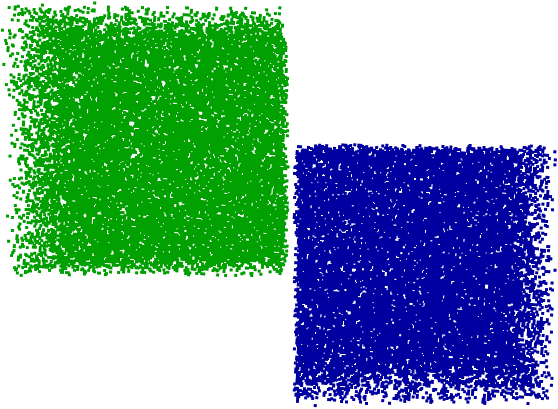
\includegraphics[height=4cm]{./figures/sec/geometrical_reasoning/blocks.png}
    \caption{Two blocks serve as an example for geometric reasoning. Here, one is interested in which direction the green cube can be moved without touching the blue one.}
    \label{fig:sec_enriched_geometricalreasoning_approach_overview_blocks}
  \end{subfigure}
  \hfill
  \begin{subfigure}[]{0.55\textwidth}
    \centering
    \begin{tikzpicture}[gnuplot]
%% generated with GNUPLOT 5.2p2 (Gentoo revision r0) (Lua 5.1; terminal rev. 99, script rev. 102)
%% Fri 15 Jun 2018 09:58:01 AM CEST
\path (0.000,0.000) rectangle (8.400,3.400);
\gpcolor{color=gp lt color axes}
\gpsetlinetype{gp lt axes}
\gpsetdashtype{gp dt axes}
\gpsetlinewidth{0.50}
\draw[gp path] (2.361,0.985)--(2.361,3.091);
\gpcolor{color=gp lt color border}
\gpsetlinetype{gp lt border}
\gpsetdashtype{gp dt solid}
\gpsetlinewidth{1.00}
\draw[gp path] (2.361,0.985)--(2.361,1.165);
\draw[gp path] (2.361,3.091)--(2.361,2.911);
\node[gp node center] at (2.361,0.677) {$5$};
\gpcolor{color=gp lt color axes}
\gpsetlinetype{gp lt axes}
\gpsetdashtype{gp dt axes}
\gpsetlinewidth{0.50}
\draw[gp path] (4.131,0.985)--(4.131,3.091);
\gpcolor{color=gp lt color border}
\gpsetlinetype{gp lt border}
\gpsetdashtype{gp dt solid}
\gpsetlinewidth{1.00}
\draw[gp path] (4.131,0.985)--(4.131,1.165);
\draw[gp path] (4.131,3.091)--(4.131,2.911);
\node[gp node center] at (4.131,0.677) {$10$};
\gpcolor{color=gp lt color axes}
\gpsetlinetype{gp lt axes}
\gpsetdashtype{gp dt axes}
\gpsetlinewidth{0.50}
\draw[gp path] (5.900,0.985)--(5.900,3.091);
\gpcolor{color=gp lt color border}
\gpsetlinetype{gp lt border}
\gpsetdashtype{gp dt solid}
\gpsetlinewidth{1.00}
\draw[gp path] (5.900,0.985)--(5.900,1.165);
\draw[gp path] (5.900,3.091)--(5.900,2.911);
\node[gp node center] at (5.900,0.677) {$15$};
\draw[gp path] (0.768,3.091)--(0.768,0.985)--(7.847,0.985)--(7.847,3.091)--cycle;
\node[gp node center,rotate=-270] at (0.276,2.038) {Count};
\node[gp node center] at (4.307,0.215) {Binned distance [a.u.]};
\gpfill{rgb color={0.667,0.000,0.000}} (0.856,0.985)--(1.034,0.985)--(1.034,1.324)--(0.856,1.324)--cycle;
\gpcolor{rgb color={0.667,0.000,0.000}}
\draw[gp path] (0.856,0.985)--(0.856,1.323)--(1.033,1.323)--(1.033,0.985)--cycle;
\gpfill{rgb color={0.667,0.000,0.000}} (1.210,0.985)--(1.388,0.985)--(1.388,1.924)--(1.210,1.924)--cycle;
\draw[gp path] (1.210,0.985)--(1.210,1.923)--(1.387,1.923)--(1.387,0.985)--cycle;
\gpfill{rgb color={0.667,0.000,0.000}} (1.564,0.985)--(1.742,0.985)--(1.742,2.323)--(1.564,2.323)--cycle;
\draw[gp path] (1.564,0.985)--(1.564,2.322)--(1.741,2.322)--(1.741,0.985)--cycle;
\gpfill{rgb color={0.000,0.667,0.000}} (1.918,0.985)--(2.096,0.985)--(2.096,2.527)--(1.918,2.527)--cycle;
\gpcolor{rgb color={0.000,0.667,0.000}}
\draw[gp path] (1.918,0.985)--(1.918,2.526)--(2.095,2.526)--(2.095,0.985)--cycle;
\gpfill{rgb color={0.000,0.667,0.000}} (2.272,0.985)--(2.450,0.985)--(2.450,2.474)--(2.272,2.474)--cycle;
\draw[gp path] (2.272,0.985)--(2.272,2.473)--(2.449,2.473)--(2.449,0.985)--cycle;
\gpfill{rgb color={0.000,0.667,0.000}} (2.626,0.985)--(2.804,0.985)--(2.804,2.279)--(2.626,2.279)--cycle;
\draw[gp path] (2.626,0.985)--(2.626,2.278)--(2.803,2.278)--(2.803,0.985)--cycle;
\gpfill{rgb color={0.000,0.667,0.000}} (2.980,0.985)--(3.158,0.985)--(3.158,2.043)--(2.980,2.043)--cycle;
\draw[gp path] (2.980,0.985)--(2.980,2.042)--(3.157,2.042)--(3.157,0.985)--cycle;
\gpfill{rgb color={0.000,0.667,0.000}} (3.334,0.985)--(3.512,0.985)--(3.512,1.811)--(3.334,1.811)--cycle;
\draw[gp path] (3.334,0.985)--(3.334,1.810)--(3.511,1.810)--(3.511,0.985)--cycle;
\gpfill{rgb color={0.000,0.667,0.000}} (3.688,0.985)--(3.866,0.985)--(3.866,1.603)--(3.688,1.603)--cycle;
\draw[gp path] (3.688,0.985)--(3.688,1.602)--(3.865,1.602)--(3.865,0.985)--cycle;
\gpfill{rgb color={0.000,0.667,0.000}} (4.042,0.985)--(4.220,0.985)--(4.220,1.431)--(4.042,1.431)--cycle;
\draw[gp path] (4.042,0.985)--(4.042,1.430)--(4.219,1.430)--(4.219,0.985)--cycle;
\gpfill{rgb color={0.000,0.667,0.000}} (4.396,0.985)--(4.574,0.985)--(4.574,1.289)--(4.396,1.289)--cycle;
\draw[gp path] (4.396,0.985)--(4.396,1.288)--(4.573,1.288)--(4.573,0.985)--cycle;
\gpfill{rgb color={0.000,0.667,0.000}} (4.750,0.985)--(4.928,0.985)--(4.928,1.167)--(4.750,1.167)--cycle;
\draw[gp path] (4.750,0.985)--(4.750,1.166)--(4.927,1.166)--(4.927,0.985)--cycle;
\gpfill{rgb color={0.000,0.667,0.000}} (5.104,0.985)--(5.282,0.985)--(5.282,1.080)--(5.104,1.080)--cycle;
\draw[gp path] (5.104,0.985)--(5.104,1.079)--(5.281,1.079)--(5.281,0.985)--cycle;
\gpfill{rgb color={0.000,0.667,0.000}} (5.458,0.985)--(5.636,0.985)--(5.636,1.031)--(5.458,1.031)--cycle;
\draw[gp path] (5.458,0.985)--(5.458,1.030)--(5.635,1.030)--(5.635,0.985)--cycle;
\gpfill{rgb color={0.000,0.667,0.000}} (5.812,0.985)--(5.990,0.985)--(5.990,1.006)--(5.812,1.006)--cycle;
\draw[gp path] (5.812,0.985)--(5.812,1.005)--(5.989,1.005)--(5.989,0.985)--cycle;
\gpfill{rgb color={0.000,0.667,0.000}} (6.166,0.985)--(6.344,0.985)--(6.344,0.993)--(6.166,0.993)--cycle;
\draw[gp path] (6.166,0.985)--(6.166,0.992)--(6.343,0.992)--(6.343,0.985)--cycle;
\gpfill{rgb color={0.000,0.667,0.000}} (6.520,0.985)--(6.698,0.985)--(6.698,0.988)--(6.520,0.988)--cycle;
\draw[gp path] (6.520,0.985)--(6.520,0.987)--(6.697,0.987)--(6.697,0.985)--cycle;
\gpfill{rgb color={0.000,0.667,0.000}} (6.874,0.985)--(7.052,0.985)--(7.052,0.986)--(6.874,0.986)--cycle;
\draw[gp path] (6.874,0.985)--(7.051,0.985)--cycle;
\gpfill{rgb color={0.000,0.667,0.000}} (7.228,0.985)--(7.406,0.985)--(7.406,0.986)--(7.228,0.986)--cycle;
\draw[gp path] (7.228,0.985)--(7.405,0.985)--cycle;
\gpfill{rgb color={0.000,0.667,0.000}} (7.582,0.985)--(7.760,0.985)--(7.760,0.986)--(7.582,0.986)--cycle;
\draw[gp path] (7.582,0.985)--(7.759,0.985)--cycle;
\gpcolor{color=gp lt color border}
\draw[gp path] (0.768,3.091)--(0.768,0.985)--(7.847,0.985)--(7.847,3.091)--cycle;
%% coordinates of the plot area
\gpdefrectangularnode{gp plot 1}{\pgfpoint{0.768cm}{0.985cm}}{\pgfpoint{7.847cm}{3.091cm}}
\end{tikzpicture}
%% gnuplot variables

    \caption{First, the distances from all voxels of the green block to all voxels from the blue block are binned. In the next step all voxels of the green block, which are below the maximum of the histogram (marked in red) are taken into account.}
    \label{fig:sec_enriched_geometricalreasoning_approach_overview_histogram}
  \end{subfigure}\\
  \begin{subfigure}[]{0.4\textwidth}
    \centering
    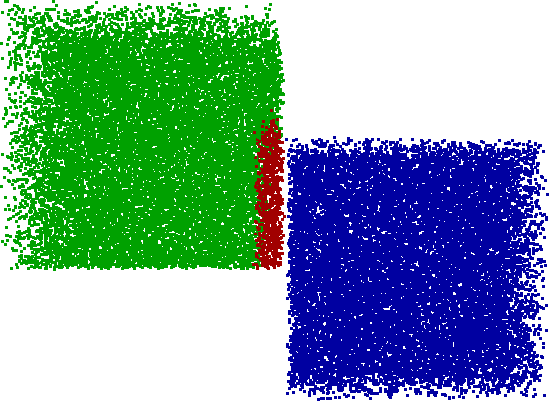
\includegraphics[height=4cm]{./figures/sec/geometrical_reasoning/blocks_marked.png}
    \caption{The voxels found in \figref{fig:sec_enriched_geometricalreasoning_approach_overview_histogram} are marked in red. Normals of these voxels are computed and k-means clustering of the normals is performed (here: $k=2$).}
    \label{fig:sec_enriched_geometricalreasoning_approach_overview_blocksmarked}
  \end{subfigure}
  \hfill
  \begin{subfigure}[]{0.55\textwidth}
    \centering
    % Define block styles
\tikzstyle{block} = [draw, rectangle, text centered, text width=6em, minimum height=5em, rounded corners=true, fill=white, fill opacity=0.9]
\tikzstyle{blockEmpty} = [rectangle, text centered, minimum height=1em, rounded corners=true, fill=white]
\tikzstyle{arrowtext} = [text width=4em, text centered]
\tikzstyle{arrow} = [draw, -latex]
\usetikzlibrary{shapes,backgrounds,calc}

\definecolor{red1}{RGB}{160,0,0}
\definecolor{green1}{RGB}{0,160,0}
\definecolor{blue1}{RGB}{0,0,160}

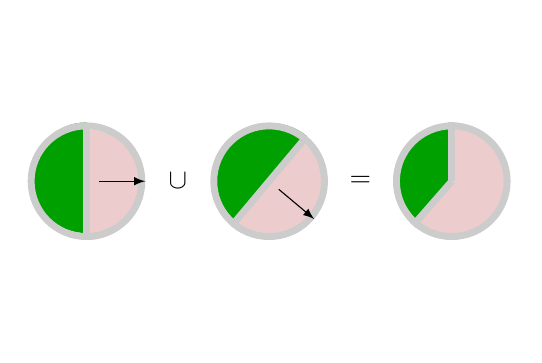
\begin{tikzpicture}[node distance=3.3em, auto]
  	% circle left
  	\node[shape=circle split,draw=gray!40,line width=0.25em,minimum size=4em, rotate=270] (circle2) {};
	\begin{scope}[on background layer]
    	\fill[red1!20, rotate=270] (circle2.base) (circle2.east) arc (0:180:2em)--cycle;
	    \fill[green1, rotate=270] (circle2.base) (circle2.west) arc (180:360:2em)--cycle;  
	\end{scope}
	\draw [arrow] (circle2.base) to (circle2.north);

	% +
	\node[right of=circle2] (plus) {$\cup$};

	% circle right
  	\node[right of=plus, shape=circle split,draw=gray!40,line width=0.25em,minimum size=4em, rotate=230] (circle1) {};
	\begin{scope}[on background layer]
    	\fill[red1!20, rotate=230] (circle1.base) (circle1.east) arc (0:180:2em)--cycle;
	    \fill[green1, rotate=230] (circle1.base) (circle1.west) arc (180:360:2em)--cycle;  
	\end{scope}
	\draw [arrow] (circle1.base) to (circle1.north);

	% =
	\node[right of=circle1] (equal) {=};

	% result
  	\node[right of=equal, shape=circle,draw=gray!40,line width=0.25em,minimum size=4em] (circle3) {};
	\draw[shape=line,draw=gray!40,line width=0.25em] (circle3.base) -- (circle3.north);
	\draw[shape=line,draw=gray!40,line width=0.25em] (circle3.base) -- ++(-1.4em, -1.6em);
	\begin{scope}[on background layer]
	    \fill[green1] (circle3.base) (circle3.north) ++(0.0em, -0.2em) arc (90:270:2em)--cycle;  
    	\fill[red1!20] (circle3.base) (circle3.south) ++(-1.3em, 0.5em) arc (-130:50:2em)--cycle;
	    \fill[red1!20, rotate=270] (circle3.base) (circle3.north) arc (180:0:2em)--cycle;  
	\end{scope}

    % Height of graphic should be 3cm, so it aligns with other subfigure
  	\node[right of=equal, rectangle, text centered, text width=0cm, minimum height=3.9cm, fill=white, node distance=0.3cm] (heightestimator) {};
\end{tikzpicture}

    \caption{A half sphere around each of the $k=2$ resulting vectors is spawned (here: half circle for visualization) and the union of all spheres is computed. The union, above marked in red, marks the ``forbidden'' directions.}
    \label{fig:sec_enriched_geometricalreasoning_approach_overview_clusterdirections}
  \end{subfigure}
  \caption{Step-by-step explanation of the geometric reasoning algorithm.}
  \label{fig:sec_enriched_geometricalreasoning_approach_overview}
\end{figure}

A step-by step explanation is shown in \figref{fig:sec_enriched_geometricalreasoning_approach_overview}.
For visualization purposes the relative position of two cubes to each other is analyzed: one green and one blue.
In a very simple approach, one could reduce the objects to one point in space, for example its mean or average position.
This, however, will ignore object sizes as well as shapes.
Instead, a more general solution, which does not depend on object size, shape, or distance is sought.
First, the distance from each voxel from one cube to each voxel in the other cube is computed and binned as shown in \figref{fig:sec_enriched_geometricalreasoning_approach_overview_blocks} and \figref{fig:sec_enriched_geometricalreasoning_approach_overview_histogram}.
For two symmetrical objects a Poisson shaped distribution is to be expected.
All voxels, which are below the first maximum and belong to the green cube are taken into consideration; these points are marked red in the histogram.
The corresponding voxels are marked in \figref{fig:sec_enriched_geometricalreasoning_approach_overview_blocksmarked} in red, too.
Next, the normals of these voxels are calculated.
These normals will, as per definition, point away from the green cube and will always point towards the blue cube.
These normals are clustered using a k-means clustering algorithms.
While undersegmentation will be harmful --- as not all directions are found --- but oversegmentation is not, a $k$ that is greater than the expected number of directions is used.
It was found heuristically that $k \approx 8$ leads to good results for most real-world examples.
Lastly, a half sphere around each resulting cluster is spawned (half circle in 2d as shown in the example in \figref{fig:sec_enriched_geometricalreasoning_approach_overview_clusterdirections}).
The union of all spheres points to the blocked directions, which is marked in red in the example --- the direction where the blue cube is located at.
This computation is performed for each object, which is in a certain radius around the \emph{main} object.
The radius is hardware dependent and defined by how much space the robot hand needs to safely grasp or push an object.

One could now devise a library of actions: Each action is combined with a robot-hardware specific set of trajectories.
Parameters, which are needed for execution, \ie where an object is located or from what angle it is safe to approach, can be generated in an automated manner by the here proposed geometric reasoning algorithm.
One such library for the Kuka Lightweight Robot was developed in collaboration with this work and published in~\cite{aeinaksoytamosiunaite2013}.
This library will be used during the next sections for action execution.
However, before one proceeds to the execution phase, one needs to analyze the structural information of \glspl{ac:esec} in more detail.
